\documentclass[12pt]{amsart}

% ============================================================
% Basic spacing
% ============================================================
\setlength{\lineskip}{0pt}

% ============================================================
% Packages for mathematics
% ============================================================
\PassOptionsToPackage{no-math}{fontspec}
\usepackage{luatexja}
\usepackage{luatexja-fontspec}
\setmainjfont{HaranoAjiMincho-Regular.otf}[BoldFont=HaranoAjiMincho-Bold.otf]
\setsansjfont{HaranoAjiGothic-Medium.otf}[BoldFont=HaranoAjiGothic-Bold.otf]
\usepackage{booktabs}
\usepackage{amsmath}
\usepackage{mathtools}
\usepackage{amssymb}
\usepackage{amsthm}
\usepackage{amscd}
\usepackage{mathrsfs}
% dsfont unavailable; its unused macro uses mathbb below.
% bbm unavailable and unused in this manuscript.

% ============================================================
% Graphics
% Use the following line for pLaTeX/upLaTeX + dvipdfmx.
% If you compile with pdfLaTeX or LuaLaTeX, remove the option [dvipdfmx].
% For PNG/JPG files with dvipdfmx, run extractbb if LaTeX cannot find the bounding box.
% ============================================================
%\usepackage[dvipdfmx]{graphicx}
\usepackage{graphicx} % Use this instead for pdfLaTeX or LuaLaTeX.

% ============================================================
% Packages for colors and text decorations
% ============================================================
\usepackage[dvipsnames]{xcolor}
% ulem unavailable and unused in this manuscript.
\usepackage{comment}

% ============================================================
% Packages for tables, lists, and diagrams
% ============================================================
\usepackage{multirow}
\usepackage{bigdelim}
\usepackage{enumerate}
\usepackage{enumitem}
% Unused legacy xypdf driver removed for LuaLaTeX; TikZ retained.
\usepackage{tikz}





% ============================================================
% tcolorbox settings
% Use as: \begin{tcolorbox}[mybox] ... \end{tcolorbox}
% ============================================================
\usepackage[most]{tcolorbox}
\tcbuselibrary{breakable, skins, theorems}
\tcbset{
  mybox/.style={
    colback=white,
    colframe=green!35!black,
    fonttitle=\bfseries,
    breakable=true
  }
}



% ============================================================
% Draft tools
% Comment out showkeys before submitting to a journal or arXiv.
% ============================================================
\usepackage[final]{showkeys} % Use this when you want to hide all labels.
%\usepackage{showkeys} % Use this when you want to show labels.
\renewcommand*{\showkeyslabelformat}[1]{%
  \begingroup
  \fboxsep=2pt%
  \fboxrule=0.3pt%
  \fbox{%
    \parbox{1.8cm}{%
      \raggedright
      \normalfont\tiny\sffamily
      \strut #1\strut
    }%
  }%
  \endgroup
}
%

% ============================================================
% This setting makes every enumerate environment use labels of the form (1), (2), (3), ...
% ============================================================

\usepackage{enumitem}
\setlist[enumerate]{label=$(\arabic*)$}

% ============================================================
% Hyperlinks
% Load hyperref near the end of the package list.
% Use the first line for pLaTeX/upLaTeX + dvipdfmx.
% If you compile with pdfLaTeX or LuaLaTeX, use the second line instead.
% ============================================================
%\usepackage[dvipdfmx,colorlinks,linkcolor=red,anchorcolor=blue,citecolor=blue]{hyperref}
\usepackage[colorlinks,linkcolor=red,anchorcolor=blue,citecolor=blue]{hyperref}



% ============================================================
% Page layout
% ============================================================
\setlength{\topmargin}{-0.25cm}
\setlength{\textwidth}{15cm}
\setlength{\textheight}{22.6cm}
\setlength{\headheight}{1em}
\setlength{\headsep}{0.5cm}
\setlength{\oddsidemargin}{0.40cm}
\setlength{\evensidemargin}{0.40cm}
\setlength{\baselineskip}{15pt}
\setlength{\footskip}{32pt}

% ============================================================
% Theorem environments
% ============================================================
\newtheorem{thm}{Theorem}[section]
\newtheorem{theo}[thm]{Theorem}
\newtheorem{cor}[thm]{Corollary}
\newtheorem{prop}[thm]{Proposition}
\newtheorem{conj}[thm]{Conjecture}
\newtheorem*{mainthm}{Theorem}

\newtheorem{deflem}[thm]{Definition-Lemma}
\newtheorem{lem}[thm]{Lemma}

\theoremstyle{definition}
\newtheorem{defn}[thm]{Definition}
\newtheorem{propdefn}[thm]{Proposition-Definition}
\newtheorem{lemdefn}[thm]{Lemma-Definition}
\newtheorem{thmdefn}[thm]{Theorem-Definition}
\newtheorem{eg}[thm]{Example}
\newtheorem{ex}[thm]{Example}
\newtheorem{exa}[thm]{Example}
\newtheorem{ques}[thm]{Question}
\newtheorem{remin}[thm]{Reminder}

\theoremstyle{remark}
\newtheorem{rem}[thm]{Remark}
\newtheorem{setup}[thm]{Setup}
\newtheorem{obs}[thm]{Observation}
\newtheorem{notation}[thm]{Notation}
\newtheorem{claim}[thm]{Claim}
\newtheorem{assup}[thm]{Assumption}
\newtheorem{cln}[thm]{Claim}

% Independent theorem-like environments.
\newtheorem{cl}{Claim}
\newtheorem{step}{Step}
\newtheorem{case}{Case}

% Unnumbered theorem-like environments.
\newtheorem*{clproof}{Proof of Claim}
\newtheorem*{ack}{Acknowledgements}

% Number equations by section.
\numberwithin{equation}{section}

% ============================================================
% Mathematical operators
% ============================================================
\newcommand{\rk}{\operatorname{rk}}
\newcommand{\rank}{\operatorname{rank}}
\newcommand{\degree}{\operatorname{deg}}
\newcommand{\codim}{\operatorname{codim}}
\newcommand{\nd}{\operatorname{nd}}

\newcommand{\Supp}{\operatorname{Supp}}
\newcommand{\supp}{\operatorname{Supp}}
\newcommand{\Rad}{\operatorname{Rad}}
\newcommand{\Exc}{\operatorname{Exc}}
\newcommand{\Div}{\operatorname{div}}

\newcommand{\End}{\operatorname{End}}
\newcommand{\eend}{\operatorname{End}}
\newcommand{\Coker}{\operatorname{Coker}}
\newcommand{\GL}{\operatorname{GL}}

\newcommand{\Hom}{\mathscr{H}\!\mathit{om}}
\newcommand{\SheafHom}[1]{\mathscr{H}\!\mathit{om}_{#1}}
\newcommand{\PGL}{\mathbb{P}\GL(r,\C)}

\DeclareMathOperator{\Ric}{Ric}
\DeclareMathOperator{\Vol}{Vol}
\DeclareMathOperator{\tr}{tr}
\DeclareMathOperator{\Id}{Id}
\DeclareMathOperator{\res}{res}
\DeclareMathOperator{\length}{length}
\DeclareMathOperator{\Homop}{Hom}
\DeclareMathOperator{\Diff}{Diff}
\DeclareMathOperator{\Lie}{Lie}
\DeclareMathOperator{\Autop}{Aut}
\DeclareMathOperator{\Kerop}{Ker}
\DeclareMathOperator{\Imageop}{Im}


% Additional template macros 

\newcommand{\MY}{\operatorname{MY}}
\newcommand{\abs}[1]{\left\lvert#1\right\rvert}
\newcommand{\norm}[1]{\left\|#1\right\|} 
\newcommand{\Rm}{\operatorname{Rm}}
\newcommand{\Cal}{\operatorname{Cal}}
\newcommand{\NA}{\operatorname{NA}}

\newcommand{\cA}{\mathcal{A}}
\newcommand{\cB}{\mathcal{B}}
\newcommand{\cC}{\mathcal{C}}
\newcommand{\cD}{\mathcal{D}}
\newcommand{\cE}{\mathcal{E}}
\newcommand{\cF}{\mathcal{F}}
\newcommand{\cG}{\mathcal{G}}
\newcommand{\cH}{\mathcal{H}}
\newcommand{\cI}{\mathcal{I}}
\newcommand{\cJ}{\mathcal{J}}
\newcommand{\cK}{\mathcal{K}}
\newcommand{\cL}{\mathcal{L}}
\newcommand{\cM}{\mathcal{M}}
\newcommand{\cN}{\mathcal{N}}
\newcommand{\cO}{\mathcal{O}}
\newcommand{\cP}{\mathcal{P}}
\newcommand{\cQ}{\mathcal{Q}}
\newcommand{\cR}{\mathcal{R}}
\newcommand{\cS}{\mathcal{S}}
\newcommand{\cT}{\mathcal{T}}
\newcommand{\cU}{\mathcal{U}}
\newcommand{\cW}{\mathcal{W}}
\newcommand{\cX}{\mathcal{X}}
\newcommand{\cY}{\mathcal{Y}}
\newcommand{\cZ}{\mathcal{Z}}

% ============================================================
% Standard maps and geometric notation
% ============================================================
\DeclareMathOperator{\pr}{pr}
\DeclareMathOperator{\id}{id}
\DeclareMathOperator{\Sym}{Sym}

\DeclareMathOperator{\Alb}{Alb}
\newcommand{\verti}{\mathrm{vert}}
\newcommand{\hor}{\mathrm{hor}}
\newcommand{\univ}{\mathrm{univ}}
\newcommand{\reg}{\mathrm{reg}}
\newcommand{\sing}{\mathrm{sing}}
\newcommand{\qt}{\mathrm{qt}}
\newcommand{\can}{\mathrm{can}}
\newcommand{\loc}{\mathrm{loc}}

\newcommand{\orb}{\mathrm{orb}}
\DeclareMathOperator{\tor}{Tor}
\newcommand{\Tor}{\mathrm{tor}}

\newcommand{\Sha}{\operatorname{Sha}}
\newcommand{\sha}{\operatorname{sha}}
\newcommand{\Shaf}{\mathrm{Sha}}
\newcommand{\shaf}{\mathrm{sha}}

% ============================================================
% Differential-geometric notation
% ============================================================
\newcommand{\ddbar}{\frac{\sqrt{-1}}{2\pi} \partial \bar{\partial}}
\newcommand{\deldel}{\sqrt{-1}\partial \overline{\partial}}
\newcommand{\dbar}{\overline{\partial}}

\newcommand{\pdrv}[2]{\frac{\partial #1}{\partial #2}}
\newcommand{\drv}[2]{\frac{d #1}{d#2}}
\newcommand{\ppdrv}[3]{\frac{\partial #1}{\partial #2 \partial #3}}

\newcommand{\polar}{\Omega}

% ============================================================
% Sheaves, ideals, automorphisms, kernels, and images
% ============================================================
\newcommand{\sO}{\mathcal{O}}
\newcommand{\mO}{\mathcal{O}}
\newcommand{\cV}{\mathcal{V}}
\newcommand{\I}[1]{\mathcal{I}(#1)}
\newcommand{\Aut}[1]{\Autop(#1)}
\newcommand{\Ker}[1]{\Kerop(#1)}
\newcommand{\Image}[1]{\Imageop(#1)}

% ============================================================
% Number systems and standard spaces
% ============================================================
\newcommand{\R}{\mathbb{R}}
\newcommand{\Z}{\mathbb{Z}}
\newcommand{\N}{\mathbb{N}}
\newcommand{\C}{\mathbb{C}}
\newcommand{\Q}{\mathbb{Q}}
\newcommand{\D}{\mathbb{D}}
\newcommand{\mP}{\mathbb{P}}
\newcommand{\B}{\mathbb{B}}
\newcommand{\T}{\mathbb{T}}
\newcommand{\G}{\mathbb{G}}

% ============================================================
% Chern character, Todd class, Chow groups, and volumes
% ============================================================
\DeclareMathOperator{\ch}{ch}
\DeclareMathOperator{\td}{td}
\DeclareMathOperator{\Td}{Td}
\DeclareMathOperator{\CH}{CH}
\DeclareMathOperator{\vol}{vol}
\DeclareMathOperator{\Amp}{Amp}
\DeclareMathOperator{\Cone}{Cone}
\newcommand{\dR}{\mathrm{dR}}

% ============================================================
% Special symbols and formatting shortcuts
% ============================================================
%\newcommand{\tl}{\hspace{-0.8ex}<\hspace{-0.8ex}}
%\newcommand{\tr}{\hspace{-0.8ex}>}

\newcommand{\xb}[1]{\textcolor{blue}{#1}}
\newcommand{\xr}[1]{\textcolor{red}{#1}}
\newcommand{\xm}[1]{\textcolor{magenta}{#1}}

% This command places a short explanation below an equality or inequality sign.
% Example: A \underalign{\text{by Lemma 1.1}}{=} B.
\newcommand{\underalign}[2]{\quad \underset{\mathclap{\strut #1}}{#2}\quad}



% Minimal repairs of the uploaded amsart template; LuaLaTeX only.
\pdfvariable minorversion=7
\theoremstyle{definition}
\newtheorem{jthm}[thm]{定理}
\newtheorem{jlem}[thm]{補題}
\newtheorem{jprop}[thm]{命題}
\setcounter{tocdepth}{1}
\emergencystretch=2em
\allowdisplaybreaks
\title[Virtual tightness on M(5,2)]{Virtual tightness on $M(5,2)$:\\
A lens-space reduction and an explicit double cover}
\author{chatGPT 6 Astra}
\date{10 September 2026}
\subjclass[2020]{Primary 57K33; Secondary 57K32}
\keywords{tight contact structure, virtually overtwisted, lens space,
Whitehead link, finite cover, convex surface}
\hypersetup{pdftitle={Virtual tightness on M(5,2)},pdfauthor={chatGPT 6 Astra}}
\begin{document}
\begin{abstract}
We determine the virtual tightness of the three positive cooriented tight contact structures on the particular Whitehead filling $M(5,2)$ of Min--Nonino. The underlying manifold is the lens space $L(10,3)$, not a hyperbolic manifold. The unique $\Psi$-structure $\xi_2$ has $c_1=0$ and becomes overtwisted in the connected double cover $L(5,3)\to L(10,3)$. The two $\Phi$-structures are universally tight. In fact every nontrivial connected cover of $\xi_2$ is overtwisted, and the minimum detecting degree is two. We give peripheral and group computations, recover the relevant surgery data, and explain why the local pieces $N_2(1)$ and $N_2(\infty)$ do not detect this phenomenon. The overtwistedness proof uses the complete tight classification upstairs, not the converse of contact-invariant vanishing. These conclusions are consequences of previously established lens-space results; this manuscript does not claim an independently new theorem.
\end{abstract}
\maketitle
\tableofcontents

\xr{This note was generated by ChatGPT 6. Iwai has NOT verified any of its mathematical content. It may therefore contain mathematical errors and should be read with caution. A Japanese version is provided below.}

\section{Introduction}\label{en-intro}
Write $M=M(5,2)$ with exactly the handed Whitehead diagram and the positive smooth surgery coefficients in Min--Nonino \cite{en-MN}. Let $\xi_2$ be their unique $\Psi$-structure, as named in their Section 5. Denote their two $\Phi$-structures by $\xi_\Phi^+$ and $\xi_\Phi^-$. The superscripts only distinguish the two structures; a choice of generator made below fixes their order.

\begin{thm}[Complete classification for the specified case]\label{en-main}
There is an oriented identification $M\cong L(10,3)$. With the pullback orientation on every cover, the following table holds:
\begin{center}
\begin{tabular}{lll}\toprule
Structure & Virtual tightness & Every connected cover of degree $>1$\\\midrule
$\xi_2$ ($\Psi$) & virtually overtwisted & overtwisted\\
$\xi_\Phi^+$ ($\Phi$) & universally tight & tight\\
$\xi_\Phi^-$ ($\Phi$) & universally tight & tight\\\bottomrule
\end{tabular}
\end{center}
The connected double cover, defined by
\begin{equation}\label{en-character}
\chi:H_1(M)=\Z/5\langle\mu\rangle\oplus\Z/2\langle\nu\rangle\longrightarrow\Z/2,
\qquad \chi(\mu)=0,\quad\chi(\nu)=1,
\end{equation}
has total space $L(5,3)$ and overtwisted pullback of $\xi_2$. Its degree is minimal among finite covers detecting overtwistedness.
\end{thm}

The result corrects an essential premise of the proposed research problem: the smallest specified example is an exceptional, spherical filling. In particular it cannot provide a new hyperbolic $L$-space example. The lens-space identification is already a specialization of Kadokami--\allowbreak Maruyama--\allowbreak Shimozawa \cite[Theorem 1.2(B)(5)]{en-KMS}. Honda's classification \cite{en-Honda} then determines the contact structures. Even the small detecting cover falls within Fossati's covering theorem \cite[Theorem 5]{en-Fossati}. We retain the explicit calculation because it identifies the families in Min--Nonino's notation and makes every step of the proposed finite-cover conclusion checkable. Its status is a proved application of known results, not a novelty claim.

\section{Preliminaries on contact three-manifolds}\label{en-prelim}
All contact structures are positive and cooriented. Thus $\xi=\ker\alpha$ with $\alpha\wedge d\alpha>0$, and the oriented real plane bundle $\xi$ has $c_1(\xi)=e(\xi)\in H^2(M;\Z)$. A structure is tight when it has no overtwisted disk. It is universally tight when its pullback to the universal cover is tight, and virtually overtwisted when it is tight but has an overtwisted pullback to a finite cover. Here the universal cover itself is finite. The tight/overtwisted alternative is also stated explicitly in Eliashberg \cite[Theorem 1.4.1]{en-Eliashberg}.

An overtwisted disk lifts to an embedded overtwisted disk under any covering: restrict the covering to the simply connected disk, choose a lift of one point, and use the lifting property. The lift is injective because its composition with the covering is the original embedding. Consequently universally tight structures have tight pullbacks under every cover. No assertion that Stein fillability implies universal tightness is used.

Our lens convention is Honda's: $L(p,q)$ is the oriented boundary of the negative linear plumbing for $-p/q$, where $p>q>0$. Equivalently we can use the usual free cyclic quotient of $S^3\subset\C^2$. Replacing $q$ by its inverse modulo $p$ gives the same oriented lens space. Reversing orientation replaces $q$ by $p-q$.

A contact coefficient is measured from the contact framing. A contact $\pm1$-surgery on a null-homologous Legendrian knot has smooth coefficient $\operatorname{tb}\pm1$. For a negative Legendrian surgery chain with matrix $Q$, the Chern class is represented in $\operatorname{coker}Q$ by the vector of rotation numbers; this follows from Gompf \cite[Proposition 2.3]{en-Gompf} and restriction to the boundary. We use Honda \cite[Theorem 2.1 and Section 4.6.2]{en-Honda} for the completeness of these chains, not merely for the existence of examples.

For convex boundary tori, a primitive vector $(p,q)$ in the exterior meridian--longitude basis has Min--Nonino slope $p/q$. In an intrinsic meridian--longitude basis of a solid torus, Honda writes slope as longitude coefficient divided by meridian coefficient. We display the basis change before using his classification. A basic slice is a minimally twisting tight $T^2\times I$ with two dividing curves on each boundary and Farey-adjacent boundary slopes. Its sign refers to the relative Euler class, after fixing coherent orientations. Within a continued fraction block, slices can be shuffled; the number of positive signs, rather than their order, is the isotopy datum. We only use the two-dividing-curve statements of Honda. The appended erratum concerning nonrotative outer layers is not used.

\section{The Min--Nonino manifolds and the exceptional filling}\label{en-manifold}
\subsection{What the specified results say at $(5,2)$}
In the published version, $\Phi(2)=\Psi(2)=1$. Theorem 1.2 and Corollary 1.4 give three isotopy classes. Theorem 1.6 gives Stein fillability. Theorem 1.7 gives the lower bound $1+2-6=-3$, hence no positive information here, and Remark 1.8 records the limitation of that argument. Proposition 3.2 supplies the single $\Psi$ class from Figure 8; Proposition 3.6 separates it from the two Figure 10 classes. Section 4 uses $M=C_5\cup N_2$, with normal boundary slopes $1$ or $\infty$; Lemma 4.7 and Theorem 4.8 give the upper bound $1+2=3$. Section 5 identifies $\xi_2$ and its Figure 31 open book. These statements were checked in the published paper, where the figure numbers differ from the early arXiv version \cite{en-MN}.

\subsection{Smooth topology and conventions}
Kadokami--\allowbreak Maruyama--\allowbreak Shimozawa's Whitehead link $W_1$ has the same handedness: positive $1$ filling on one component produces the right-handed trefoil exterior. Their Theorem 1.2(B)(5) says that a filling with second coefficient $2$ and first coefficient $p_1/q_1$ is a lens filling when $|p_1-4q_1|=1$, and gives
\[
L(2p_1,8q_1-p_1)
\]
in their \emph{positive} unknot-surgery convention. Substituting $p_1=5,q_1=1$ gives $L(10,3)$ in that convention. Their Section 5, Figure 4, proves this using a $(2,4)$-torus-link surgery presentation; it is a topological surgery calculation, not a numerical identification \cite{en-KMS}.

Changing to Honda's negative-surgery convention gives $L(10,7)$. Since $3\cdot7\equiv1\pmod {10}$, it is oriented diffeomorphic to $L(10,3)$ in our convention. Also $3^2\equiv-1\pmod {10}$, so this particular lens space is amphicheiral. Thus the possible global orientation convention cannot change the asserted oriented diffeomorphism type here. We still keep the induced positive contact orientation throughout.

The original linking matrix and its cokernel are
\begin{equation}\label{en-homology}
Q_W=\begin{pmatrix}5&0\\0&2\end{pmatrix},\qquad
H_1(M;\Z)=\Z/5\langle\mu\rangle\oplus\Z/2\langle\nu\rangle\cong\Z/10.
\end{equation}
The zero off-diagonal entries use the Whitehead link's algebraic linking number zero. This is the specialization of the homology computation in the proof of Min--Nonino's Proposition 3.6. As an independent linking-pairing check, $Q_W^{-1}$ evaluates on $\mu+\nu$ to $1/5+1/2=7/10$. The inverse matrix of the negative $[-4,-2,-2]$ chain evaluates on its first meridian to $-3/10\equiv7/10$. A common global sign in the convention for boundary linking pairings cancels in this comparison.

\subsection{A peripheral group calculation}
Here is a direct algebraic check using the once-punctured-torus description, retaining the full mapping class. Take $\pi_1(\Sigma)=\langle x,y\rangle$, $c=[x,y]$, and based twists
\[
A(x)=xy^{-1},\quad A(y)=y,\qquad B(x)=x,\quad B(y)=yx.
\]
Both preserve $c$. Their matrices are
\[
A=\begin{pmatrix}1&0\\-1&1\end{pmatrix},\qquad
B=\begin{pmatrix}1&1\\0&1\end{pmatrix}.
\]
The word $\phi_5=ABA^4$ in Section 5 of \cite{en-MN} gives
\[
\phi_5(x)=x^{-3}y^{-1},\qquad \phi_5(y)=yxy^{-1},\qquad
(\phi_5)_*=\begin{pmatrix}-3&1\\-1&0\end{pmatrix}.
\]
Choose the stable-letter and oriented peripheral conventions so that $\mu_2=t$, $\lambda_2=c$ and the filling relation is $t^2c=1$. The compatible mapping-torus presentation, with based loops transported in this convention, is
\begin{equation}\label{en-group}
G=\langle x,y,t\mid txt^{-1}=x^{-3}y^{-1},\quad
tyt^{-1}=yxy^{-1},\quad t^2[x,y]=1\rangle.
\end{equation}
The peripheral pair is part of this presentation; it must not be recovered from the matrix alone. Changing the stable-letter direction requires changing the peripheral convention with it.

For completeness the simplification is entirely explicit. Since $c=t^{-2}$,
\[
yxy^{-1}=c^{-1}x=t^2x,\quad y=txt,\quad tx^2t=x^{-3}.
\]
Set $z=tx^2$. Then $z^2=x^{-1}$, so
\begin{equation}\label{en-tietze}
x=z^{-2},\qquad t=z^5,\qquad y=z^8.
\end{equation}
The commutator is now trivial and the filling relation says $z^{10}=1$. Conversely these three substitutions in a cyclic group of order ten satisfy every relation in \eqref{en-group}, and $tx^2=z$. Thus $G\cong\Z/10$, with the meridian $t$ of the $2$-filled component equal to the unique order-two element. This agrees with the independent lens-surgery identification, which already proves $\pi_1(M)=\Z/10$.

The dual core $K_*$ of the $2$ filling has the class $\pm t=z^5$. Indeed a core longitude can be chosen as $(-1,0)$ complementary to the filling meridian $(2,1)$. The core has order \emph{two}, not infinite order. Nontriviality of its class cannot be used to obtain arbitrarily large unwrapping degree.

\section{The three tight structures on \texorpdfstring{$M(5,2)$}{M(5,2)}}\label{en-three}
\subsection{Recovering the two surgery descriptions}
The specialization of Min--Nonino Figure 8 has four chain unknots $L'_1,\ldots,L'_4$, each with $\operatorname{tb}=-1$, $\operatorname{rot}=0$, and contact coefficient $-1$. The trefoil $L_0$ has $\operatorname{tb}=1$, $\operatorname{rot}=0$, and contact coefficient $r-1=+1$. Thus the smooth coefficients are $-2,-2,-2,-2,+2$. No stabilization choice occurs at $r=2$. The $-2$ chain has continued fraction $-5/4=[-2,-2,-2,-2]$.

In Figure 10 the trefoil has contact coefficient $n-1=4$, and the other component has coefficient $-1/(r-1)=-1$. Converting the positive coefficient uses $4/(1-4)=-4/3=[-2,-2,-2]$: the first trefoil has rotation zero and the three further push-offs have rotation numbers $\varepsilon,\varepsilon,\varepsilon$, where $\varepsilon=\pm1$ is the single stabilization choice. The other component has rotation zero. Min--Nonino's Proposition 3.6 tracks their meridians under the handle slides and gives
\begin{equation}\label{en-c1MN}
c_1(\xi_2)=0,\qquad
\operatorname{PD}c_1(\xi_\Phi^\varepsilon)=\varepsilon,3\mu.
\end{equation}
In the first equality one can also apply directly their contact $\pm1$-surgery Chern-class formula: every entry in the rotation vector is zero. We do not incorrectly treat the positive-surgery handlebody as Stein.

\begin{figure}[htbp]\centering
\includegraphics[height=5.7cm]{figures/mn_fig8.pdf}\hspace{1cm}
\includegraphics[height=4.2cm]{figures/mn_fig10.pdf}
\caption{The relevant fronts in the published Figures 8 and 10 of Min--Nonino. Read the left with $n-1=4$, $r-1=1$, and the right with $n-1=4$, $-1/(r-1)=-1$. The ellipsis is exactly the four-unknot chain described in the text. Reproduced as cropped, unaltered figure excerpts from \cite{en-MN}, copyright the authors, CC BY 4.0, \url{https://creativecommons.org/licenses/by/4.0/}.}\label{en-fronts}
\end{figure}

\subsection{The lens-space chain and its signs}
For $L(10,3)$ the surgery chain is
\[
-10/3=[-4,-2,-2],\qquad
Q_{10}=\begin{pmatrix}-4&1&0\\1&-2&1\\0&1&-2\end{pmatrix}.
\]
\begin{center}
\begin{tikzpicture}[baseline=0]
\draw[thick] (0,0)--(3,0)--(6,0);
\foreach \xx/\ww in {0/-4,3/-2,6/-2}{
\filldraw[fill=white,thick] (\xx,0) circle (0.12);
\node[above] at (\xx,.18) {$\ww$};}
\node[below] at (0,-.2) {$\operatorname{rot}\in\{-2,0,2\}$};
\node[below] at (3,-.2) {$\operatorname{rot}=0$};
\node[below] at (6,-.2) {$\operatorname{rot}=0$};
\end{tikzpicture}
\end{center}
This is the plumbing graph of a linear Hopf chain; each edge means linking number $+1$, every contact coefficient is $-1$, and the smooth weights are the vertex labels. It is not a purported contact handle-slide sequence from Figure 8. The contact identification is instead proved by the complete classification and the Chern calculation.

Let $h_i$ be the meridians. The relations give
\[
h_2=4h_1,\quad h_3=7h_1,\quad10h_1=0.
\]
Put $g=\operatorname{PD}^{-1}(h_1)$. Honda's complete list and Gompf's formula give
\begin{center}
\begin{tabular}{cccc}\toprule
First-unknot stabilizations & Rotation vector & $c_1$ & Identification\\\midrule
two negative & $(-2,0,0)$ & $-2g$ & one $\Phi$ structure\\
one of each sign & $(0,0,0)$ & $0$ & $\xi_2$\\
two positive & $(2,0,0)$ & $2g$ & the other $\Phi$ structure\\\bottomrule
\end{tabular}
\end{center}
These Chern classes are distinct modulo ten. In particular the zero-class tight structure is unique, making its identification with $\xi_2$ independent of the chosen diffeomorphism to the lens space.

In the associated Honda decomposition the effective continued fraction block has two sign choices, represented by $--$, $+-$ (equivalently $-+$), and $++$; the $-2$ vertices add no stabilization choices. One can see the block as the Farey-adjacent path $-1,-2,-3$ in Honda's coordinates. More explicitly $p'=3,q'=1$ solve $10q'-3p'=1$, and the reduced boundary slope in Honda's Proposition 4.17 is $-p'/q'=-3=[-4,-2,-1]$. This gives the two basic slices in that block. Reversing all auxiliary orientations interchanges $+$ and $-$ but preserves the distinction between mixed and uniform signs. Honda's Proposition 5.1(3), with its proof, identifies the two uniform-sign structures as universally tight. The next section gives a separate proof detecting the mixed-sign structure in a specific double cover.

\section{Finite covers and convex decompositions}\label{en-covers}
\subsection{The cover as a quotient and as a filling}
Let $\zeta=e^{2\pi i/10}$ and
\[
\rho(z_1,z_2)=(\zeta z_1,\zeta^3z_2),\qquad (z_1,z_2)\in S^3.
\]
The action is free: a fixed point of $\rho^k$ with either coordinate nonzero requires respectively $10\mid k$ or $10\mid3k$, hence $10\mid k$. Its subgroup $\langle\rho^2\rangle$ has order five. Therefore
\begin{equation}\label{en-covermap}
q:S^3/\langle\rho^2\rangle=L(5,3)\longrightarrow
S^3/\langle\rho\rangle=L(10,3),\qquad [u]\longmapsto[u]
\end{equation}
is a connected, unbranched, orientation-preserving double cover. Transfer it through an oriented identification with $M$. It equals the cover \eqref{en-character}, since a cyclic group of order ten has exactly one index-two subgroup. This also removes any dependence on the choice of lens-space identification.

There is a direct filling construction. On $C_5$ the character records the mapping-torus direction modulo two. Its cover is the mapping torus of $\phi_5^2$; its boundary lattice is generated by $(2,0),(0,1)$ in the downstairs $(t,c)$ basis. The filling meridian $(2,1)$ is in this lattice and has upstairs coordinates $(1,1)$. Choose upstairs longitude $(-1,0)$ and downstairs longitude $(-1,0)$. The boundary map $\operatorname{diag}(2,1)$ sends the upstairs meridian to the downstairs meridian and the upstairs longitude to twice the downstairs longitude. In these intrinsic solid-torus coordinates the map is therefore
\[
D^2\times S^1\longrightarrow D^2\times S^1,\qquad(w,u)\longmapsto(w,u^2).
\]
It is unbranched, extends the boundary map, and maps the core with degree two. In particular this construction covers the \emph{filled} manifold, not just the exterior.

All connected covers correspond to subgroups $\langle z^d\rangle$ of $\Z/10$, with $d\mid10$. The degree of the lift of the core in a degree-$d$ cover is the order of $z^5$ in $\Z/d$, namely $d/\gcd(d,5)$. Thus:
\begin{center}
\begin{tabular}{cccc}\toprule
Cover degree & Total space & Components over $K_*$ & Degree on each core\\\midrule
1 & $L(10,3)$ & 1 & 1\\
2 & $L(5,3)$ & 1 & 2\\
5 & $L(2,1)$ & 5 & 1\\
10 & $S^3$ & 5 & 2\\\bottomrule
\end{tabular}
\end{center}
This table exhausts every connected finite cover and every possible degree, not just a low-index experiment. Every finite quotient of the fundamental group is cyclic of order dividing ten.

\subsection{Why the local solid tori do not become overtwisted}
Take $m=(2,1)$ and $\ell=(-1,0)$ on $\partial N_2$. The basis matrix and inverse are
\begin{equation}\label{en-basis}
P=\begin{pmatrix}2&-1\\1&0\end{pmatrix},\qquad
P^{-1}=\begin{pmatrix}0&1\\-1&2\end{pmatrix}.
\end{equation}
The dividing vectors at slopes $1$ and $\infty$ become respectively $(1,1)$ and $(0,-1)$ in the intrinsic $(m,\ell)$ basis. Each has geometric intersection one with $m$. For the first, replace $\ell$ by $\ell+2m$; for the second, reverse the dividing vector and replace $\ell$ by $\ell+m$. The resulting vector is $(-1,1)$ in each case, hence Honda slope $-1$. With two dividing curves there is exactly one tight solid-torus structure with this boundary datum, and it is universally tight \cite[Proposition 5.1(2), the $s=-1$ case]{en-Honda}. There is no nontrivial continued fraction block with mixed signs in either normalized $N_2$ piece.

For the double cover a primitive vector $(p,q)$ closes after $k=2/\gcd(2,p)$ turns, and lifts to $(kp/2,kq)$. In the exterior basis upstairs this gives
\begin{center}
\begin{tabular}{cccc}\toprule
Curve downstairs & Vector & Turns & Lifted vector\\\midrule
filling meridian & $(2,1)$ & 1 & $(1,1)$\\
slope $1$ dividing curve & $(1,1)$ & 2 & $(1,2)$\\
slope $\infty$ dividing curve & $(1,0)$ & 2 & $(1,0)$\\\bottomrule
\end{tabular}
\end{center}
In both boundary cases each of the two dividing curves has a single connected lift; there are still two dividing curves. Its determinant with the upstairs meridian has absolute value one. Thus the lifted solid torus is again standard and tight, also following from universal tightness downstairs. The overtwisted disk established below cannot be contained entirely in this $N_2$ lift.

The decomposition torus is not $\pi_1$-injective in $M$: its group is infinite and $\pi_1(M)$ is finite; indeed it bounds a solid torus. No incompressible-torus gluing theorem can simply convert tight or universally tight restrictions here into universal tightness of the closed manifold. Section 5 of Min--Nonino cannot detect this case merely by counting non-universally-tight restrictions on $N_2$. Also its unwrapping language must not be interpreted as allowing arbitrary unwrapping of this order-two core.

\section{Virtual overtwistedness}\label{en-vot}
\begin{lem}\label{en-upstairs}
No positive cooriented tight contact structure on $L(5,3)$ has zero first Chern class.
\end{lem}
\begin{proof}
The expansion $-5/3=[-2,-3]$ has exactly two tight structures by Honda's Theorem 2.1. Both are realized by the negative Legendrian chain with matrix
\[
Q_5=\begin{pmatrix}-2&1\\1&-3\end{pmatrix},
\]
and their rotation vectors are $(0,1)$ and $(0,-1)$. In its cokernel let $k_1,k_2$ be the meridians. The relations $-2k_1+k_2=0$ and $k_1-3k_2=0$ give $k_2=2k_1$ and $5k_1=0$. The determinant is five, so $k_1$ has order exactly five. Gompf's formula now gives $\operatorname{PD}c_1=\pm k_2=\pm2k_1$, both nonzero. Completeness of Honda's list excludes any additional zero-class tight structure.
\end{proof}

\begin{prop}\label{en-doubleOT}
The particular double cover $\pi$ defined by \eqref{en-character} has overtwisted pullback $\pi^*\xi_2$.
\end{prop}
\begin{proof}
By \eqref{en-c1MN}, $c_1(\xi_2)=0$. The differential of a covering identifies the oriented plane bundle of the pulled-back contact structure with the pullback bundle. Hence
\[
c_1(\pi^*\xi_2)=\pi^*c_1(\xi_2)=0.
\]
The cover is positive and its total space is $L(5,3)$. If $\pi^*\xi_2$ were tight, Lemma \ref{en-upstairs} would force its first Chern class to be nonzero, a contradiction. It is therefore overtwisted. Since $\xi_2$ itself is tight, it is virtually overtwisted.
\end{proof}

This proves existence of an overtwisted disk in a specified closed finite cover by a complete classification obstruction. It does not give a parametrized disk or a sequence of bypasses on a chosen diagram. Such extra geometric data are not needed for the implication: tightness is exactly absence of such a disk, and every possible tight structure upstairs has been excluded. In particular no assertion of the form ``mixed signs should become overtwisted'' or ``$c(\xi)=0$ implies overtwisted'' occurs in this proof.

\section{Proof of the main theorem and reverse checks}\label{en-proof}
\begin{proof}[Proof of Theorem \ref{en-main}]
The oriented lens-space identification was established in Section \ref{en-manifold}. Min--Nonino gives exactly the three indicated structures. The Chern computations and Honda's complete chain identify them with the three entries of the table in Section \ref{en-three}. The two uniform-sign entries are universally tight by Honda's Proposition 5.1(3); therefore they have tight pullbacks to every cover. The zero-class entry is $\xi_2$, and Proposition \ref{en-doubleOT} detects it in degree two. Independently of sign identifications, Honda gives exactly two universally tight classes on $L(10,3)$; after excluding $\xi_2$, they must be the two $\Phi$ classes. This rechecks the secondary conclusion. No degree-one cover detects overtwistedness because the structure downstairs is tight.

There are only the three nontrivial connected cover degrees $2,5,10$. A disk in the degree-two cover lifts to $S^3$, so the degree-ten pullback is overtwisted. For degree five the total space is $L(2,1)=\R P^3$. Its unique positive tight contact structure is universally tight (Honda's Theorem 2.1 and Proposition 5.1(3), with $q=p-1$). If the degree-five pullback were tight, its universal pullback to $S^3$ would therefore be tight. But that is the same universal pullback of $\xi_2$ just shown to be overtwisted. This contradiction settles degree five and completes every entry of the theorem.
\end{proof}

The requested reverse audit has four precise answers. The detecting cover is the unique connected index-two cover $\ker\chi$, explicitly \eqref{en-covermap}. It covers $M$ because the peripheral filling meridian lifts primitively and the map extends over the attached solid torus. The contact structure upstairs is defined as $\pi^*\xi_2$; its Chern class is computed by naturality, not by selecting an arbitrary plane field on the cover. An overtwisted disk is forced by Lemma \ref{en-upstairs} and the tight/overtwisted alternative. Thus no unstated gluing hypothesis or virtual-to-finite passage remains.

Additional error checks are useful. The map is unbranched; it is unrelated to a cyclic branched cover of a transverse knot. The order of $K_*$ is two, so a degree-five cover does not unwrap it at all. The comparison is between oriented Chern classes on oriented covers; changing a generator can multiply a class by a unit but cannot turn zero into nonzero. The two Chern residues upstairs are $2,3$ modulo five, not $\pm1$ in the first-meridian generator. The base coefficient $2$ is smooth, whereas the Figure 8 trefoil's contact coefficient is $+1$. The negative chain coefficients used in the lens classification are smooth. Finally, the two universally tight structures here contradict neither the hyperbolic assumption of the original conjecture nor any theorem of Min--Nonino: $M$ is spherical.

\section{Other routes and further consequences}\label{en-further}
\subsection{The Figure 31 open book}
The original open book of $L(5,4)$ has once-punctured-torus page and monodromy $\phi_5=D_\alpha D_\beta D_\alpha^4$. The surgered Figure 31 page has genus one and two boundary components. On that page Min--Nonino gives
\begin{equation*}\begin{aligned}
\widetilde\phi_5&=D_\alpha D_\beta D_\alpha^4D_\gamma^{-1}\Delta,\\
\Delta&=D_\gamma D_\alpha^{-2}D_\delta D_\sigma,\\
\widetilde\phi_5&=D_\alpha D_\beta D_\alpha^2D_\delta D_\sigma.
\end{aligned}\end{equation*}
Here $\Delta$ twists positively about both boundary components, $\alpha$ and $\gamma$ are disjoint, and the curves and the factorization are the ones used in their Section 5. This is a specialization of their existing positive factorization. The right-veering property is consistent with tightness and follows from the positive factorization. It supplies no assertion about universal tightness. The fractional Dehn twist bound $0<c(\phi_5)<1$ in Section 4.1 concerns the \emph{one}-boundary page, not the two-boundary monodromy $\widetilde\phi_5$. Its $2\times2$ homology matrix cannot be used to read off both boundary coefficients of $\widetilde\phi_5$.

\begin{figure}[htbp]\centering
\includegraphics[width=.92\textwidth]{figures/mn_fig31.pdf}
\caption{The pages and twist curves from Min--Nonino Figure 31, specialized by setting $n-1=4$. Cropped, unaltered excerpt of \cite{en-MN}, copyright the authors, CC BY 4.0. The full monodromy, including both boundary twists, is specified in the text.}\label{en-openbook}
\end{figure}

A covering of the smooth mapping torus does not automatically give a lift of every twist in this factorization to a chosen page cover. In particular we have not claimed a non-right-veering lifted monodromy, computed the two boundary fractional coefficients, or asserted a destabilization. Those are not hypotheses or missing steps in the completed finite-cover proof.

\subsection{Heegaard Floer invariants and comparison of methods}
Ozsv\'ath--Szab\'o \cite[Theorems 1.4 and 1.5]{en-OS} prove, respectively, that an overtwisted contact structure has zero contact invariant and that a Stein fillable contact structure has nonzero invariant. Thus the three base structures have nonzero contact invariants by Min--Nonino's fillability theorem, whereas the three nontrivial connected pullbacks of $\xi_2$ have zero invariant by the theorem proved above. The vanishing upstairs is a \emph{consequence}, not the overtwistedness test. No unrestricted covering naturality theorem for the contact invariant is being assumed. The ordinary first Chern class, whose naturality is immediate, suffices.

The four proposed routes therefore have different outcomes. The local convex-solid-torus route finds only standard universally tight restrictions and cannot settle the global structure alone. The surgery/finite-cover route gives an exhaustive covering list and, combined with the tight classification on the double cover, completes the proof. The open-book route verifies the existing fillability factorization. The Heegaard Floer route checks consistency but needs no new covering map on Floer homology. Etnyre--Honda's punctured-torus normalizations \cite[Section 5.2, Proposition 5.5 and Lemma 5.7]{en-EH} and Conway--Min's surgery arguments \cite[Section 5.2]{en-CM} explain the methods behind Min--Nonino's Section 4; they are not used to impose an unjustified incompressible gluing argument in this exceptional closed filling.

One immediate consequence is a counterexample to the proposed statement that all three structures on $M(5,2)$ might be virtually overtwisted. Exactly two are universally tight. Another is a completely determined unwrapping profile: no cover of this manifold unwraps $K_*$ more than twice, despite the existence of a degree-ten universal cover.

\section{Novelty audit}\label{en-novelty}
\subsection{Novelty statement}
\begin{enumerate}
\item Min--Nonino proves the number three, the two surgery families, their distinction, and Stein fillability. Their general lower bound for virtual overtwistedness is ineffective at $(5,2)$; their Remark 1.8 is a limitation of that treatment, not evidence that every listed integer case escapes older lens-space classification.
\item The smooth identification is explicitly contained in Kadokami--\allowbreak Maruyama--\allowbreak Shimozawa's lens-surgery theorem. Honda already classifies all three tight structures and their universal tightness on the resulting lens space.
\item The contribution of this manuscript is the explicit specialization, the identification of $\xi_2$ by its zero Chern class, the concrete double cover, and the complete verification of its finite-cover behavior. These are proved here, but are consequences of existing theorems. No independently new mathematical theorem has been established in this execution.
\item A search need not locate an article with the identical notation to refute novelty. Fossati's Theorem 5 says that a virtually overtwisted structure on $L(p,q)$ becomes overtwisted in a degree-$d$ cover when $q<p<dq$ (and such a cover exists). Use the oriented equivalent description $L(10,7)$: $7<10<14$. It already subsumes the double-cover assertion, and also applies with $d=5$. Thus even the detecting degree is covered by prior work. We expressly do not claim ``no prior theorem was found.''
\end{enumerate}

\subsection{Search scope and the current hyperbolic literature}
The audit date is 10 September 2026. Searches combined the phrases ``Whitehead link contact structures'', ``M(n,2) contact structure'', ``universally tight Whitehead surgery'', ``virtually overtwisted Whitehead link'', ``hyperbolic L-space universally tight'', ``finite covers tight contact structures'', and ``Hyunki Min Isacco Nonino'', together with exact $M(5,2)$ and $L(10,3)$ variants. We checked accessible arXiv records and PDFs, publisher records, author publication lists, reference lists, and indexed scholarly/citation searches. MathSciNet was not available through an authenticated subscription; zbMATH-targeted searches gave no decisive additional item, and a direct Google Scholar profile request was rate-limited. We therefore do not pretend that an exhaustive subscription-database citation search was performed. The positive discovery of older encompassing theorems makes an absence-of-results argument unnecessary.

Hyunki Min's and Isacco Nonino's publication lists were checked \cite{en-websites}. The 2026 preprint on transverse knots and cyclic \emph{branched} covers and the 2025 preprint on contact surgery distance were screened by their records; they do not replace the unbranched lens-cover argument here. Nonino's 2026 thesis, deposited on 8 September 2026, provides a particularly recent account of the context \cite{en-thesis}.

There is a substantive update to the conjectural background. Baldwin--Sivek--Zung \cite[Theorem 1.4]{en-BSZ} already gives hyperbolic $L$-spaces with universally tight contact structures (their $r>4g$ surgery result). Nonino's thesis explicitly discusses this change. Thus the original equivalence in Min--Nonino's Conjecture 1.1 should not be treated as an unrefuted conjecture as of this audit. This update is logically independent of our theorem: the present $M(5,2)$ is not hyperbolic in the first place.

For source verification, the original Honda text including its erratum, the Min--Nonino published text and requested figures, Kadokami--\allowbreak Maruyama--\allowbreak Shimozawa's theorem and sufficiency proof, Fossati's theorem and covering discussion, Gompf's Chern formula, and the indicated Ozsv\'ath--Szab\'o, Eliashberg, Etnyre--Honda and Conway--Min passages were read. Giroux's publisher metadata was checked and the convex-surface discussion was consulted in Daniel Mathews's complete English translation \cite{en-Giroux}; no unverified theorem number from the inaccessible publisher original is cited. Martelli's exceptional-filling tables were also checked as a topological consistency comparison \cite{en-Martelli}.

The requested independent-new-theorem condition has therefore not been met. The specified primary and secondary virtual-tightness questions have both been settled rigorously in this manuscript. No open case for these three structures is left as a conjectural substitute. We make no new claim about the genuinely different manifolds $M(n,2)$ for $n>5$.

\section*{Computational appendix}\addcontentsline{toc}{section}{Computational appendix}
The accompanying \texttt{compute\_m52.py} uses exact rational and integer arithmetic and optionally SnapPy 3.3.2. Its output is saved in \texttt{computation\_results.json}. The experiment suggested the cyclic lens-space reduction; the group simplification, older lens-surgery theorem, and Chern-class proof then replaced that experiment by human-checkable arguments. All finite quotients are exhausted algebraically, so no bounded computational search is being presented as an exhaustive theorem for an infinite group.

For reproducibility the Whitehead PD code used in the experiment is
\begin{verbatim}
[(0,5,1,6), (4,1,5,2), (2,8,3,7),
 (8,0,9,3), (6,4,7,9)]
\end{verbatim}
with primitive filling pairs \texttt{[(5,1),(2,1)]}. This is the mirror of SnapPy's default \texttt{L5a1} convention. As a convention check, \texttt{[(5,1),(5,2)]} identifies the Weeks filling \texttt{m003(-3,1)} and has experimental volume $0.9427073628$, as required by Min--Nonino's Corollary 1.5. Nonprimitive input pairs describe a different object and were excluded. Neither a near-zero numerical volume nor software recognition is used as a proof.

The essential exact-arithmetic check is short:
\begin{verbatim}
from fractions import Fraction as F
assert -4-1/(F(-2)-1/F(-2)) == F(-10,3)
assert -2-1/F(-3) == F(-5,3)
# First-meridian generators in the two chain cokernels:
h10 = [1,4,7]                 # modulo 10
h5  = [1,2]                   # modulo 5
c1_base = [r % 10 for r in (-2,0,2)]
c1_tight_upstairs = [(2*r) % 5 for r in (-1,1)]
assert 0 in c1_base and 0 not in c1_tight_upstairs
\end{verbatim}
The full code also verifies the free-group automorphism words, reverse cyclic substitutions, boundary determinants, and every connected cover/core degree.

\renewcommand{\refname}{References}
\addcontentsline{toc}{section}{References}
\begin{thebibliography}{99}
\bibitem{en-MN}
H. Min and I. Nonino, \emph{Tight contact structures on a family of hyperbolic $L$-spaces}, Geometriae Dedicata \textbf{220} (2026), article 45. Published 4 July 2026. \href{https://doi.org/10.1007/s10711-026-01097-8}{doi:10.1007/s10711-026-01097-8}. Earlier version: \href{https://arxiv.org/abs/2311.14103}{arXiv:2311.14103}.

\bibitem{en-KMS}
T. Kadokami, N. Maruyama and M. Shimozawa, \emph{Lens surgeries along the $n$-twisted Whitehead link}, \href{https://arxiv.org/abs/1205.2311}{arXiv:1205.2311} (2012). Theorem 1.2 and Section 5 of the 24-page version.

\bibitem{en-Honda}
K. Honda, \emph{On the classification of tight contact structures I}, Geometry \& Topology \textbf{4} (2000), 309--368; erratum, \textbf{5} (2001), 1501--1514. \href{https://arxiv.org/abs/math/9910127}{arXiv:math/9910127v3}, with appended erratum.

\bibitem{en-Fossati}
E. Fossati, \emph{Topological constraints for Stein fillings of tight structures on lens spaces}, \href{https://arxiv.org/abs/1906.09162}{arXiv:1906.09162}, version 3 (2020). Theorem 5 and Section 4.

\bibitem{en-Gompf}
R. E. Gompf, \emph{Handlebody construction of Stein surfaces}, Annals of Mathematics \textbf{148} (1998), 619--693. \href{https://arxiv.org/abs/math/9803019}{arXiv:math/9803019}.

\bibitem{en-Eliashberg}
Y. Eliashberg, \emph{Contact 3-manifolds twenty years since J. Martinet's work}, Annales de l'Institut Fourier \textbf{42} (1992), 165--192. \href{https://doi.org/10.5802/aif.1288}{doi:10.5802/aif.1288}.

\bibitem{en-Giroux}
E. Giroux, \emph{Convexit\'e en topologie de contact}, Commentarii Mathematici Helvetici \textbf{66} (1991), 637--677. \href{https://doi.org/10.1007/BF02566670}{doi:10.1007/BF02566670}. Text consulted through D. Mathews's translation, \emph{Convexity in Contact Topology}, 12 July 2010, \href{https://few.vu.nl/~pasquott/Giroux-convexity.pdf}{translation PDF}, especially Part II.2.

\bibitem{en-EH}
J. B. Etnyre and K. Honda, \emph{Knots and contact geometry. I. Torus knots and the figure eight knot}, Journal of Symplectic Geometry \textbf{1} (2001), 63--120. \href{https://arxiv.org/abs/math/0006112}{arXiv:math/0006112}.

\bibitem{en-CM}
J. Conway and H. Min, \emph{Classification of tight contact structures on surgeries on the figure-eight knot}, Geometry \& Topology \textbf{24} (2020), 1457--1517. \href{https://arxiv.org/abs/1901.06066}{arXiv:1901.06066}.

\bibitem{en-OS}
P. Ozsv\'ath and Z. Szab\'o, \emph{Heegaard Floer homology and contact structures}, Duke Mathematical Journal \textbf{129} (2005), 39--61. \href{https://arxiv.org/abs/math/0210127}{arXiv:math/0210127}.

\bibitem{en-Martelli}
B. Martelli, \emph{Dehn surgery on the minimally twisted seven-chain link}, Communications in Analysis and Geometry \textbf{29} (2021), 1597--1641. \href{https://arxiv.org/abs/1808.08430}{arXiv:1808.08430v2}, Table 13.

\bibitem{en-BSZ}
J. A. Baldwin, S. Sivek and J. Zung, \emph{Pseudo-Anosov flows on hyperbolic $L$-spaces}, \href{https://arxiv.org/abs/2505.21113}{arXiv:2505.21113} (2025), version 2. Theorem 1.4.

\bibitem{en-thesis}
I. Nonino, \emph{Hyperbolic $L$-spaces from a contact geometry perspective}, Ph.D. thesis, University of Glasgow, 2026; deposited 8 September 2026. \href{https://theses.gla.ac.uk/86215/}{Repository record and full thesis}.

\bibitem{en-websites}
H. Min, \href{https://hkmin27.github.io/}{author publication list}; I. Nonino, \href{https://sites.google.com/view/isaccononinomath/home-page}{author publication list}. Accessed 10 September 2026. Screened records: M. Kegel and I. Nonino, \emph{Transverse knots determined by cyclic branched covers}, \href{https://arxiv.org/abs/2603.25805}{arXiv:2603.25805}; M. Kegel, I. Nonino and M. Yadav, \emph{Contact surgery distance}, \href{https://arxiv.org/abs/2512.14904}{arXiv:2512.14904}.

\end{thebibliography}
\newpage
\begin{center}
{\Large\bfseries $M(5,2)$ 上の接触構造の virtual tightness：\\レンズ空間への帰着と明示的な二重被覆}
\medskip

chatGPT 6 Astra
\end{center}
\section*{要旨}\addcontentsline{toc}{section}{日本語版：要旨}
Min--Nonino の Whitehead link 手術多様体 $M(5,2)$ 上の三つの正の余向き付けられた tight 接触構造について、virtual tightness を完全に判定する。この多様体は双曲多様体ではなく、レンズ空間 $L(10,3)$ である。唯一の $\Psi$ 型構造 $\xi_2$ の第一 Chern 類は零であり、連結二重被覆 $L(5,3)\to L(10,3)$ への引き戻しは overtwisted になる。二つの $\Phi$ 型構造は universally tight である。さらに $\xi_2$ の非自明な連結被覆への引き戻しはすべて overtwisted であり、最小検出次数は二である。周辺群、基本群、手術図式、convex 境界の計算を与え、局所的な $N_2(1)$ および $N_2(\infty)$ からだけでは今回の現象を検出できない理由を示す。証明には被覆上の tight 構造の完全分類を用い、接触不変量の消滅の逆命題は用いない。本稿の結論は既知のレンズ空間の諸定理の帰結であり、独立した新定理とは主張しない。

\xr{このノートはchatGPT 6が生成したものであり, 岩井は数学的な検証を全く行っていません. そのため数学的な間違いがあるかもしれません. そのため注意深く読んでください.}

\section{序論}\label{ja-intro}
Min--Nonino \cite{ja-MN} の Whitehead 図式の鏡像を取り違えず、正の位相的手術係数 $(5,2)$ を用いて $M=M(5,2)$ と書く。同論文第5節で命名された唯一の $\Psi$ 型構造を $\xi_2$ とする。二つの $\Phi$ 型構造を $\xi_\Phi^+,\xi_\Phi^-$ と書く。上付き符号は二つを区別する記号であり、後述する生成元の選択によって順序が定まる。

\begin{jthm}[指定された場合の完全な判定]\label{ja-main}
向きを保つ同定 $M\cong L(10,3)$ が存在する。各被覆に引き戻しの向きを入れると、次の表が成り立つ。
\begin{center}
\begin{tabular}{lll}\toprule
接触構造 & virtual tightness & 次数 $>1$ のすべての連結被覆\\\midrule
$\xi_2$（$\Psi$ 型） & virtually overtwisted & overtwisted\\
$\xi_\Phi^+$（$\Phi$ 型） & universally tight & tight\\
$\xi_\Phi^-$（$\Phi$ 型） & universally tight & tight\\\bottomrule
\end{tabular}
\end{center}
具体的に、準同型
\begin{equation}\label{ja-character}
\chi:H_1(M)=\Z/5\langle\mu\rangle\oplus\Z/2\langle\nu\rangle\longrightarrow\Z/2,
\qquad\chi(\mu)=0,\quad\chi(\nu)=1
\end{equation}
の核に対応する連結二重被覆の全空間は $L(5,3)$ であり、$\xi_2$ の引き戻しは overtwisted である。overtwistedness を検出する有限被覆の最小次数は二である。
\end{jthm}

研究課題の前提で修正が必要なのは、最小の指定例が例外的な球面幾何の Dehn filling だという点である。従って、この例から新しい双曲 $L$-space の事例を得ることはできない。レンズ空間の同定は既に Kadokami--\allowbreak Maruyama--\allowbreak Shimozawa \cite[Theorem 1.2(B)(5)]{ja-KMS} に含まれ、Honda の分類 \cite{ja-Honda} が接触構造を決定する。小さい検出被覆さえ Fossati \cite[Theorem 5]{ja-Fossati} の範囲内にある。それでも具体的な計算を記すのは、Min--Nonino の各 family を正確に同定し、有限被覆での結論を一行ずつ確認できる形にするためである。本稿は既知結果の証明付きの応用であり、新規性を主張するものではない。

\section{三次元接触多様体の準備}\label{ja-prelim}
接触構造はすべて正で余向き付けられているとする。従って $\xi=\ker\alpha$、$\alpha\wedge d\alpha>0$ であり、向き付けられた実平面束 $\xi$ に対し $c_1(\xi)=e(\xi)\in H^2(M;\Z)$ である。overtwisted disk を含まない接触構造を tight と呼ぶ。普遍被覆への引き戻しが tight であるとき universally tight、元は tight だがある有限被覆への引き戻しが overtwisted であるとき virtually overtwisted と呼ぶ。今回の普遍被覆はそれ自身有限被覆である。tight と overtwisted の二者択一は Eliashberg \cite[Theorem 1.4.1]{ja-Eliashberg} にも明記されている。

overtwisted disk は任意の被覆に埋め込まれた overtwisted disk として持ち上がる。実際、円板が単連結なので一点の lift を指定すれば持ち上げが存在する。その持ち上げと被覆写像の合成が元の埋め込みであるため、持ち上げも単射である。従って universally tight な構造のすべての被覆への引き戻しは tight である。Stein fillable から universally tight を結論する推論は用いない。

レンズ空間の規約は Honda に合わせ、$p>q>0$ に対して $-p/q$ の負の線形 plumbing の向き付けられた境界を $L(p,q)$ とする。これは $S^3\subset\C^2$ の通常の自由巡回商でも記述できる。$q$ を法 $p$ での逆元に置き換えても、向きを保つ微分同相型は変わらない。向きの反転は $q$ を $p-q$ に置き換える。

contact surgery coefficient は接触 framing から測る。零ホモロジー的 Legendrian knot の contact $\pm1$ 手術の位相的係数は $\operatorname{tb}\pm1$ である。負の Legendrian surgery chain の行列が $Q$ のとき、第一 Chern 類は $\operatorname{coker}Q$ 内で rotation number のベクトルにより表される。これは Gompf \cite[Proposition 2.3]{ja-Gompf} と境界への制限から従う。これらの chain が全 tight 構造を尽くすことには Honda \cite[Theorem 2.1, Section 4.6.2]{ja-Honda} を用いる。単にいくつかの Stein fillable な例を作っただけでは十分ではない。

convex 境界では、外部の meridian--longitude 基底に関する原始ベクトル $(p,q)$ の Min--Nonino slope は $p/q$ である。一方、solid torus 自身の meridian--longitude 基底では、Honda slope は longitude の係数を meridian の係数で割った値である。分類を使う前に必ず基底変換を示す。basic slice とは、各境界に二本の dividing curve を持ち、両境界 slope が Farey 隣接である、minimally twisting な tight $T^2\times I$ である。その符号は向きを一貫して選んだ相対 Euler 類による。一つの continued fraction block 内では basic slice を shuffle でき、順序ではなく正符号の個数が isotopy データになる。本稿は二本の dividing curve に関する Honda の結果だけを用いる。付加された erratum の nonrotative outer layer に関する一意性は用いない。

\section{Min--Nonino 多様体と例外的 filling}\label{ja-manifold}
\subsection{指定された諸結果を $(5,2)$ に代入する}
出版版では $\Phi(2)=\Psi(2)=1$ である。Theorem 1.2 と Corollary 1.4 は三つの isotopy class を与え、Theorem 1.6 は Stein fillability を与える。Theorem 1.7 の下界は $1+2-6=-3$ となり、この場合は有効な正の情報を与えず、Remark 1.8 がその議論の限界を記している。Proposition 3.2 は Figure 8 から唯一の $\Psi$ 型を与え、Proposition 3.6 はそれを Figure 10 の二構造から区別する。第4節は $M=C_5\cup N_2$ を用い、正規化された境界 slope は $1$ または $\infty$ である。Lemma 4.7 と Theorem 4.8 は上界 $1+2=3$ を与える。第5節は $\xi_2$ と Figure 31 の open book を同定する。これらは出版版の本文と図から確認した。初期 arXiv 版とは図番号が異なる \cite{ja-MN}。

\subsection{位相型と向きの規約}
Kadokami--\allowbreak Maruyama--\allowbreak Shimozawa の Whitehead link $W_1$ は同じ handedness を持つ。一方の成分への正の $1$ filling は右手 trefoil の外部を与える。同論文 Theorem 1.2(B)(5) によれば、第2係数が $2$、第1係数が $p_1/q_1$ のとき、$|p_1-4q_1|=1$ ならばレンズ空間となり、同論文の正の unknot surgery の規約では
\[
L(2p_1,8q_1-p_1)
\]
である。$p_1=5,q_1=1$ を代入すると $L(10,3)$ となる。同論文第5節 Figure 4 の十分性の証明は、$(2,4)$-torus link の手術図式を用いている。これは数値的な認識ではなく位相的手術計算である \cite{ja-KMS}。

Honda の負の surgery の規約ではいったん $L(10,7)$ となる。しかし $3\cdot7\equiv1\pmod {10}$ なので、本稿の $L(10,3)$ と向きを保って微分同相である。また $3^2\equiv-1\pmod {10}$ より、このレンズ空間は amphicheiral である。このため大域的な向きの規約の違いによって今回主張する向き付けられた微分同相型が変わることはない。ただし接触構造には一貫して誘導された正の向きを用いる。

元の linking matrix と cokernel は
\begin{equation}\label{ja-homology}
Q_W=\begin{pmatrix}5&0\\0&2\end{pmatrix},\qquad
H_1(M;\Z)=\Z/5\langle\mu\rangle\oplus\Z/2\langle\nu\rangle\cong\Z/10
\end{equation}
である。非対角成分が零であることは Whitehead link の algebraic linking number が零であることによる。これは Min--Nonino の Proposition 3.6 の証明中のホモロジー計算の特殊化でもある。独立な linking pairing の検算として、$Q_W^{-1}$ は $\mu+\nu$ 上で $1/5+1/2=7/10$ を与える。負の $[-4,-2,-2]$ chain の逆行列は第1 meridian 上で $-3/10\equiv7/10$ を与える。境界 linking pairing の定義に伴う共通の全体符号は、この比較では相殺される。

\subsection{周辺データ付きの基本群計算}
穴あきトーラスの記述による代数的な検算を与える。行列だけでなく mapping class の語全体を保持する。$\pi_1(\Sigma)=\langle x,y\rangle$、$c=[x,y]$ とし、基点付き Dehn twist を
\[
A(x)=xy^{-1},\quad A(y)=y,\qquad B(x)=x,\quad B(y)=yx
\]
と取る。両者とも $c$ を保ち、行列は
\[
A=\begin{pmatrix}1&0\\-1&1\end{pmatrix},\qquad
B=\begin{pmatrix}1&1\\0&1\end{pmatrix}
\]
である。\cite{ja-MN} 第5節の語 $\phi_5=ABA^4$ より
\[
\phi_5(x)=x^{-3}y^{-1},\qquad \phi_5(y)=yxy^{-1},\qquad
(\phi_5)_*=\begin{pmatrix}-3&1\\-1&0\end{pmatrix}.
\]
stable letter と向き付けた周辺データを、$\mu_2=t$、$\lambda_2=c$、filling relation が $t^2c=1$ となる規約で選ぶ。この規約に従って基点付き loop を移送した整合的な mapping torus の表示は
\begin{equation}\label{ja-group}
G=\langle x,y,t\mid txt^{-1}=x^{-3}y^{-1},\quad
tyt^{-1}=yxy^{-1},\quad t^2[x,y]=1\rangle
\end{equation}
である。この表示には周辺対も含めて指定している。行列から周辺対を復元したと考えてはいけない。stable letter の向きを変える場合は周辺規約も同時に変える必要がある。

表示の簡約をすべて書く。$c=t^{-2}$ より
\[
yxy^{-1}=c^{-1}x=t^2x,\quad y=txt,\quad tx^2t=x^{-3}.
\]
$z=tx^2$ と置くと $z^2=x^{-1}$ となるので
\begin{equation}\label{ja-tietze}
x=z^{-2},\qquad t=z^5,\qquad y=z^8.
\end{equation}
従って commutator は自明となり、filling relation は $z^{10}=1$ となる。逆に、位数十の巡回群の中でこの三つの代入をすると \eqref{ja-group} の全関係式を満たし、$tx^2=z$ でもある。従って $G\cong\Z/10$ であり、$2$ filling の成分の meridian $t$ は唯一の位数二の元である。これは、既に $\pi_1(M)=\Z/10$ を与える独立なレンズ空間の手術同定とも一致する。

$2$ filling の surgery dual core $K_*$ は $\pm t=z^5$ を表す。実際、filling meridian $(2,1)$ と相補的な core longitude は $(-1,0)$ と選べる。core の位数は無限ではなく二である。その class が非自明であることから、任意に大きい次数で unwrap できるとは結論できない。

\section{\texorpdfstring{$M(5,2)$}{M(5,2)} 上の三つの tight 構造}\label{ja-three}
\subsection{二つの手術図式の復元}
Min--Nonino Figure 8 を特殊化すると、chain に四つの unknot $L'_1,\ldots,L'_4$ があり、すべて $\operatorname{tb}=-1$、$\operatorname{rot}=0$、contact coefficient $-1$ である。trefoil $L_0$ は $\operatorname{tb}=1$、$\operatorname{rot}=0$、contact coefficient $r-1=+1$ である。従って位相的係数は $-2,-2,-2,-2,+2$ となる。$r=2$ では stabilization の選択はない。$-2$ chain の連分数は $-5/4=[-2,-2,-2,-2]$ である。

Figure 10 では trefoil の contact coefficient は $n-1=4$、もう一つの成分は $-1/(r-1)=-1$ である。正の係数の変換には $4/(1-4)=-4/3=[-2,-2,-2]$ を用いる。最初の trefoil の rotation は零、残る三つの push-off の rotation number は $\varepsilon,\varepsilon,\varepsilon$ となり、$\varepsilon=\pm1$ が一度の stabilization の選択である。もう一つの成分の rotation は零である。Min--Nonino の Proposition 3.6 は handle slide における meridian の変化を追跡しており、ここに代入すると
\begin{equation}\label{ja-c1MN}
c_1(\xi_2)=0,\qquad
\operatorname{PD}c_1(\xi_\Phi^\varepsilon)=\varepsilon,3\mu
\end{equation}
を得る。最初の等式は、rotation vector の全成分が零なので、同論文の contact $\pm1$-surgery に対する Chern 類の公式から直接にも従う。正の手術を含むこの handlebody を Stein と誤認しているわけではない。

\begin{figure}[htbp]\centering
\includegraphics[height=5.7cm]{figures/mn_fig8.pdf}\hspace{1cm}
\includegraphics[height=4.2cm]{figures/mn_fig10.pdf}
\caption{出版版 Min--Nonino の Figures 8, 10 の該当 front。左は $n-1=4,r-1=1$、右は $n-1=4,-1/(r-1)=-1$ と読む。左の省略記号は本文の四つの unknot からなる chain を表す。\cite{ja-MN} の図の切り出しであり、図中の内容は変更していない。著作権は原著者、CC BY 4.0（\url{https://creativecommons.org/licenses/by/4.0/}）。}\label{ja-fronts}
\end{figure}

\subsection{レンズ空間の chain と符号}
$L(10,3)$ の surgery chain は
\[
-10/3=[-4,-2,-2],\qquad
Q_{10}=\begin{pmatrix}-4&1&0\\1&-2&1\\0&1&-2\end{pmatrix}
\]
である。
\begin{center}
\begin{tikzpicture}[baseline=0]
\draw[thick] (0,0)--(3,0)--(6,0);
\foreach \xx/\ww in {0/-4,3/-2,6/-2}{
\filldraw[fill=white,thick] (\xx,0) circle (0.12);
\node[above] at (\xx,.18) {$\ww$};}
\node[below] at (0,-.2) {$\operatorname{rot}\in\{-2,0,2\}$};
\node[below] at (3,-.2) {$\operatorname{rot}=0$};
\node[below] at (6,-.2) {$\operatorname{rot}=0$};
\end{tikzpicture}
\end{center}
これは線形 Hopf chain の plumbing graph であり、各辺は linking number $+1$、全 contact coefficient は $-1$、頂点の重みは位相的係数を表す。Figure 8 からの contact handle slide の列を示したと主張する図ではない。接触構造の同定は、完全分類と Chern 類の計算によって証明する。

meridian を $h_i$ とすると、関係式から
\[
h_2=4h_1,\quad h_3=7h_1,\quad10h_1=0
\]
を得る。$g=\operatorname{PD}^{-1}(h_1)$ と置く。Honda の完全なリストと Gompf の公式は次を与える。
\begin{center}
\begin{tabular}{cccc}\toprule
最初の unknot の stabilization & rotation vector & $c_1$ & 同定\\\midrule
二つとも負 & $(-2,0,0)$ & $-2g$ & 一方の $\Phi$ 型\\
正負一つずつ & $(0,0,0)$ & $0$ & $\xi_2$\\
二つとも正 & $(2,0,0)$ & $2g$ & 他方の $\Phi$ 型\\\bottomrule
\end{tabular}
\end{center}
三つの Chern 類は法十で相異なる。特に第一 Chern 類が零の tight 構造はただ一つであり、$\xi_2$ との同定はレンズ空間への微分同相の選び方に依存しない。

対応する Honda decomposition の有効な continued fraction block には二つの符号があり、$--$、$+-$（$-+$ と同値）、$++$ が現れる。$-2$ の頂点は stabilization の選択を加えない。この block は Honda 座標の Farey 隣接 path $-1,-2,-3$ として見られる。詳しくは、$p'=3,q'=1$ は $10q'-3p'=1$ を満たし、Honda Proposition 4.17 の簡約後の境界 slope は $-p'/q'=-3=[-4,-2,-1]$ となる。従ってこの block に二つの basic slice がある。補助的な向きをすべて反転すれば正負は入れ替わるが、混合符号か同一符号かという区別は変わらない。Honda Proposition 5.1(3) とその証明は同一符号の二構造を universally tight と同定する。次節以降では混合符号の構造を、指定した二重被覆で独立に検出する。

\section{有限被覆と convex decomposition}\label{ja-covers}
\subsection{商空間と filling による被覆の構成}
$\zeta=e^{2\pi i/10}$ とし、$S^3\subset\C^2$ 上で
\[
\rho(z_1,z_2)=(\zeta z_1,\zeta^3z_2)
\]
と定める。$\rho^k$ に固定点があるなら、零でない座標に応じて $10\mid k$ または $10\mid3k$ が必要となり、いずれも $10\mid k$ となる。従ってこの作用は自由である。部分群 $\langle\rho^2\rangle$ の位数は五なので
\begin{equation}\label{ja-covermap}
q:S^3/\langle\rho^2\rangle=L(5,3)\longrightarrow
S^3/\langle\rho\rangle=L(10,3),\qquad[u]\longmapsto[u]
\end{equation}
は連結、非分岐、向きを保つ二重被覆である。$M$ との向きを保つ同定を通してこれを移す。位数十の巡回群には指数二の部分群がただ一つなので、これは \eqref{ja-character} の被覆と同じである。このことから同定の選択にも依存しない。

filling を用いる直接の構成もある。$C_5$ 上では、$\chi$ は mapping torus 方向を法二で数える。その被覆は $\phi_5^2$ の mapping torus であり、境界の格子は下の $(t,c)$ 基底で $(2,0),(0,1)$ によって生成される。filling meridian $(2,1)$ はこの格子に属し、上では $(1,1)$ となる。上下の longitude をそれぞれ $(-1,0)$ と選ぶ。境界写像 $\operatorname{diag}(2,1)$ は上の meridian を下の meridian に、上の longitude を下の longitude の二倍に移す。従って内在的 solid torus 座標では
\[
D^2\times S^1\longrightarrow D^2\times S^1,\qquad(w,u)\longmapsto(w,u^2)
\]
と書ける。これは非分岐で境界写像を延長し、core 上の次数は二である。従って被覆しているのは外部だけでなく、filling 後の閉多様体である。

すべての連結被覆は $\Z/10$ の部分群 $\langle z^d\rangle$、$d\mid10$ に対応する。次数 $d$ の被覆で core の各 lift が持つ次数は、$z^5$ の $\Z/d$ における位数、すなわち $d/\gcd(d,5)$ である。よって次の表を得る。
\begin{center}
\begin{tabular}{cccc}\toprule
被覆次数 & 全空間 & $K_*$ 上の成分数 & 各 core 上の次数\\\midrule
1 & $L(10,3)$ & 1 & 1\\
2 & $L(5,3)$ & 1 & 2\\
5 & $L(2,1)$ & 5 & 1\\
10 & $S^3$ & 5 & 2\\\bottomrule
\end{tabular}
\end{center}
これは低次数の実験の結果だけではなく、すべての連結有限被覆と可能な次数を尽くす。基本群の任意の有限商は、位数が十を割る巡回群である。

\subsection{局所 solid torus が overtwisted にならない理由}
$\partial N_2$ で $m=(2,1)$、$\ell=(-1,0)$ とする。基底変換行列と逆行列は
\begin{equation}\label{ja-basis}
P=\begin{pmatrix}2&-1\\1&0\end{pmatrix},\qquad
P^{-1}=\begin{pmatrix}0&1\\-1&2\end{pmatrix}
\end{equation}
である。slope $1$ と $\infty$ の dividing vector は、内在的な $(m,\ell)$ 基底でそれぞれ $(1,1)$ と $(0,-1)$ になる。両方とも $m$ との幾何的交点数は一である。前者では $\ell$ を $\ell+2m$ に変え、後者では dividing vector の符号を反転して $\ell$ を $\ell+m$ に変える。どちらも $( -1,1)$ となり、Honda slope は $-1$ である。dividing curve が二本なら、この境界データに対する tight solid torus はただ一つで universally tight である \cite[Proposition 5.1(2), $s=-1$ の場合]{ja-Honda}。正規化されたどちらの $N_2$ piece にも、混合符号を持つ非自明な continued fraction block は存在しない。

二重被覆では、原始ベクトル $(p,q)$ は $k=2/\gcd(2,p)$ 周で閉じ、$(kp/2,kq)$ に持ち上がる。上の外部基底では
\begin{center}
\begin{tabular}{cccc}\toprule
下の曲線 & ベクトル & 周回数 & lift のベクトル\\\midrule
filling meridian & $(2,1)$ & 1 & $(1,1)$\\
slope $1$ の dividing curve & $(1,1)$ & 2 & $(1,2)$\\
slope $\infty$ の dividing curve & $(1,0)$ & 2 & $(1,0)$\\\bottomrule
\end{tabular}
\end{center}
となる。二つの境界の場合のいずれでも、各 dividing curve の lift は一成分で、全体で二本のままである。上の meridian との determinant の絶対値は一である。従って lift した solid torus も標準的で tight であり、これは下の universally tightness からも従う。後で存在を証明する overtwisted disk は、$N_2$ の lift 全体の内部には収まらない。

分解 torus の基本群は無限であるのに $\pi_1(M)$ は有限であり、この torus は $M$ 内で $\pi_1$-injective ではない。実際、solid torus の境界である。従って incompressible torus に沿う gluing theorem を、そのまま局所的な tightness または universally tightness から閉多様体の universally tightness を得るために使うことはできない。Min--Nonino 第5節の $N_2$ 上の non-universally-tight 制限の個数を数える方法だけでは、この場合を検出できない。また unwrap に関する記述を、この位数二の core を任意次数で unwrap できるという意味で読んではいけない。

\section{Virtual overtwistedness}\label{ja-vot}
\begin{jlem}\label{ja-upstairs}
$L(5,3)$ 上に、第一 Chern 類が零である正の余向き付けられた tight 接触構造は存在しない。
\end{jlem}
\begin{proof}[証明]
$-5/3=[-2,-3]$ なので、Honda Theorem 2.1 により tight 構造はちょうど二つである。両方とも負の Legendrian chain
\[
Q_5=\begin{pmatrix}-2&1\\1&-3\end{pmatrix}
\]
で実現され、rotation vector は $(0,1)$ と $(0,-1)$ である。cokernel の meridian を $k_1,k_2$ とする。関係式 $-2k_1+k_2=0$、$k_1-3k_2=0$ より $k_2=2k_1$、$5k_1=0$ を得る。determinant は五なので、$k_1$ の位数はちょうど五である。Gompf の公式により $\operatorname{PD}c_1=\pm k_2=\pm2k_1$ で、どちらも零ではない。Honda のリストが完全であることから、これ以外に零の Chern 類を持つ tight 構造がある可能性も排除される。
\end{proof}

\begin{jprop}\label{ja-doubleOT}
\eqref{ja-character} で定義した具体的な二重被覆 $\pi$ に対し、$\pi^*\xi_2$ は overtwisted である。
\end{jprop}
\begin{proof}[証明]
\eqref{ja-c1MN} より $c_1(\xi_2)=0$ である。被覆写像の微分により、引き戻した接触構造の向き付けられた平面束は元の平面束の引き戻しと同一視される。従って
\[
c_1(\pi^*\xi_2)=\pi^*c_1(\xi_2)=0.
\]
被覆は向きを保ち、その全空間は $L(5,3)$ である。仮に $\pi^*\xi_2$ が tight ならば、補題 \ref{ja-upstairs} により第一 Chern 類は非零となり、矛盾する。従って overtwisted である。元の $\xi_2$ は tight なので、virtually overtwisted である。
\end{proof}

この証明は、指定された閉有限被覆における overtwisted disk の存在を、完全分類による障害として証明している。円板のパラメータ表示や、特定の図式上の bypass の列を与えているわけではない。しかし tight であることはそのような円板が存在しないことと同値であり、被覆上で tight になり得るすべての構造を排除したので、結論に必要な含意は完全である。「混合符号だから多分 overtwisted になる」や「$c(\xi)=0$ だから overtwisted」という推論はこの証明には現れない。

\section{主定理の証明と逆方向からの検算}\label{ja-proof}
\begin{proof}[定理 \ref{ja-main} の証明]
向き付けられたレンズ空間の同定は第\ref{ja-manifold}節で示した。Min--Nonino により指定された三構造が全 tight 構造を尽くす。Chern 類の計算と Honda の完全な chain 分類から、それらは第\ref{ja-three}節の表の三つと同定される。同一符号の二構造は Honda Proposition 5.1(3) により universally tight であり、すべての被覆で tight のままである。零の Chern 類を持つ構造は $\xi_2$ であり、命題 \ref{ja-doubleOT} により次数二で検出される。符号の同定と独立にも、Honda によれば $L(10,3)$ 上の universally tight な isotopy class はちょうど二つなので、$\xi_2$ を排除すれば残る二つの $\Phi$ 型に一致する。この方法でも secondary target の結論を再検算できる。次数一の被覆は元の tight な構造と同じなので検出しない。

非自明な連結被覆の次数は $2,5,10$ のみである。二重被覆上の円板は $S^3$ に持ち上がるので、十重被覆への引き戻しも overtwisted である。五重被覆の全空間は $L(2,1)=\R P^3$ である。その唯一の正の tight 構造は universally tight である（Honda Theorem 2.1 と Proposition 5.1(3) の $q=p-1$ の場合）。仮に五重被覆への引き戻しが tight ならば、その普遍被覆 $S^3$ への引き戻しも tight になる。しかしこれは、既に overtwisted と示した $\xi_2$ の普遍被覆への引き戻しと同じである。この矛盾により次数五の場合も解決し、表の全項目が証明された。
\end{proof}

依頼された逆方向の監査には、次の四つの明確な答えがある。検出被覆はただ一つの連結指数二被覆 $\ker\chi$ で、具体式は \eqref{ja-covermap} である。filling meridian が原始的に lift し、接着する solid torus 上へ写像が延長するので、それは本当に $M$ の被覆である。上の接触構造は $\pi^*\xi_2$ と定義しており、その Chern 類は自然性によって計算したのであって、上に任意の平面場を選んだのではない。overtwisted disk の存在は補題 \ref{ja-upstairs} と tight/overtwisted の二者択一が保証する。従って未記載の gluing の仮定や、普遍被覆から有限被覆への未証明の移行は残っていない。

さらに次の誤りも排除した。被覆は非分岐で、transverse knot の巡回分岐被覆とは異なる。$K_*$ の位数は二なので、五重被覆では core は全く unwrap されない。比較は向き付けられた被覆上の向き付けられた Chern 類について行う。生成元の変更は unit 倍を与えるだけで、零を非零には変えない。上の第1 meridian を生成元とした Chern residue は $\pm1$ ではなく、法五で $2,3$ である。元の係数 $2$ は位相的係数であり、Figure 8 の trefoil の contact coefficient は $+1$ である。レンズ空間の負の chain に書いた係数は位相的係数である。最後に、この universally tight な二構造は、元の予想の双曲性の仮定にも Min--Nonino の定理にも反しない。今回の $M$ は球面的だからである。

\section{他の証明ルートと帰結}\label{ja-further}
\subsection{Figure 31 の open book}
$L(5,4)$ の元の open book は穴あきトーラスを page とし、monodromy は $\phi_5=D_\alpha D_\beta D_\alpha^4$ である。手術後の Figure 31 の page は genus 一で境界成分を二つ持つ。この page 上で Min--Nonino は
\begin{equation*}\begin{aligned}
\widetilde\phi_5&=D_\alpha D_\beta D_\alpha^4D_\gamma^{-1}\Delta,\\
\Delta&=D_\gamma D_\alpha^{-2}D_\delta D_\sigma,\\
\widetilde\phi_5&=D_\alpha D_\beta D_\alpha^2D_\delta D_\sigma
\end{aligned}\end{equation*}
を与える。$\Delta$ は両境界成分に沿う正の Dehn twist の積であり、$\alpha$ と $\gamma$ は交わらず、各曲線と因数分解は同論文第5節のものである。これは既存の正の因数分解の特殊化である。right-veering 性はその正の因数分解から従い、tightness と整合的であるが、universally tightness は与えない。第4.1節の fractional Dehn twist coefficient の範囲 $0<c(\phi_5)<1$ は境界が一つの page に対するものであり、境界が二つある $\widetilde\phi_5$ のものではない。その $2\times2$ のホモロジー行列から、$\widetilde\phi_5$ の二つの境界係数を読み取ることはできない。

\begin{figure}[htbp]\centering
\includegraphics[width=.92\textwidth]{figures/mn_fig31.pdf}
\caption{Min--Nonino Figure 31 の page と twist 曲線。$n-1=4$ として特殊化する。\cite{ja-MN} の内容を変更しない図の切り出し。著作権は原著者、CC BY 4.0。両境界の twist を含む完全な monodromy は本文に記した。}\label{ja-openbook}
\end{figure}

滑らかな mapping torus の被覆があることだけでは、選んだ page cover に因数分解の各 twist が lift するとは限らない。本稿では non-right-veering な lifted monodromy、二つの境界の正確な fractional coefficient、または destabilization を得たとは主張しない。これらは完成した有限被覆の証明の仮定でも、欠落した証明段階でもない。

\subsection{Heegaard Floer 不変量と方法の比較}
Ozsv\'ath--Szab\'o \cite[Theorems 1.4, 1.5]{ja-OS} は、それぞれ overtwisted なら接触不変量が零、Stein fillable なら非零であることを示す。従って元の三構造の接触不変量は Min--Nonino の fillability 定理により非零であり、$\xi_2$ の三つの非自明連結被覆での接触不変量は本稿の定理により零である。被覆上での消滅は結論であって、overtwistedness の検出原理ではない。接触不変量に対する無条件の covering naturality は仮定しない。通常の第一 Chern 類の自然性だけで十分である。

指定された四つのルートの結果は次のように整理できる。局所 convex solid torus のルートは標準的な universally tight 制限しか見いださず、それ単独では大域的構造を決定しない。手術と有限被覆のルートは全被覆を尽くし、二重被覆上の tight 分類と合わせて証明を完成する。open book のルートは既存の fillability の因数分解を確認する。Heegaard Floer のルートは整合性を確認するが、新たな Floer homology 間の被覆写像は必要ない。Etnyre--Honda の穴あきトーラスの正規化 \cite[Section 5.2, Proposition 5.5, Lemma 5.7]{ja-EH} と Conway--Min の手術に関する議論 \cite[Section 5.2]{ja-CM} は Min--Nonino 第4節の背景となるが、この例外的な閉 filling に根拠のない incompressible gluing の議論を適用するためには用いない。

直ちに得られる帰結の一つは、「$M(5,2)$ 上の三構造がすべて virtually overtwisted」という予想的な文が偽だということである。ちょうど二構造は universally tight である。もう一つは core の unwrapping が完全に決まることである。十重の普遍被覆が存在するにもかかわらず、どの被覆も $K_*$ を二回より多く unwrap しない。

\section{新規性監査}\label{ja-novelty}
\subsection{Novelty statement}
\begin{enumerate}
\item Min--Nonino は三という個数、二つの surgery family、その区別、Stein fillability を証明した。virtually overtwisted 構造の一般的下界は $(5,2)$ では有効でない。Remark 1.8 はその論文の手法の限界であり、列挙された整数係数の場合がすべて過去のレンズ空間分類の範囲外にあるという証拠ではない。
\item 位相的な同定は Kadokami--\allowbreak Maruyama--\allowbreak Shimozawa の lens surgery の定理に明示的に含まれる。得られたレンズ空間上の三 tight 構造とその universally tightness は、既に Honda の分類が決定する。
\item 本稿で実際に行ったことは、具体的特殊化、零 Chern 類による $\xi_2$ の同定、明示的二重被覆、全有限被覆における挙動の検算である。これらには証明を与えたが、既存定理の帰結である。今回の実行で独立した新しい数学的定理を得たとは主張しない。
\item 新規性を否定するために全く同じ記号を使う論文が見つかる必要はない。Fossati の Theorem 5 は、$q<p<dq$ のとき、$L(p,q)$ 上の virtually overtwisted 構造が次数 $d$ の被覆で overtwisted になることを示す（その被覆が存在する場合）。向きを保って同値な $L(10,7)$ を用いると $7<10<14$ であり、二重被覆の主張は既に含まれる。$d=5$ にも適用できる。従って検出次数の結果も先行研究の範囲内であり、「同じ定理は見つからなかった」とは主張しない。
\end{enumerate}

\subsection{検索の範囲と最新の双曲多様体の文献}
監査日は2026年9月10日である。検索では ``Whitehead link contact structures'', ``M(n,2) contact structure'', ``universally tight Whitehead surgery'', ``virtually overtwisted Whitehead link'', ``hyperbolic L-space universally tight'', ``finite covers tight contact structures'', ``Hyunki Min Isacco Nonino'' を組み合わせ、さらに $M(5,2)$ と $L(10,3)$ の完全一致の変種も用いた。アクセス可能な arXiv の書誌と PDF、出版社の書誌、著者の論文リスト、引用文献表、学術・引用検索のインデックスを確認した。MathSciNet の認証済み購読アクセスはなく、zbMATH を対象とする検索では決定的な追加項目を得られず、Google Scholar の profile への直接アクセスは rate limit に遭った。従って購読データベースの被引用文献を完全に網羅したとは記さない。既に結論を包含する過去の定理を積極的に発見したので、検索結果の不在を新規性の根拠にする必要はない。

Hyunki Min と Isacco Nonino の論文リストを確認した \cite{ja-websites}。2026年の transverse knot と巡回分岐被覆に関する preprint、および2025年の contact surgery distance の preprint は書誌を確認したが、今回の非分岐レンズ空間被覆の議論に取って代わるものではない。2026年9月8日に登録された Nonino の学位論文は、特に新しい時点の背景を与える \cite{ja-thesis}。

予想の背景には重要な更新がある。Baldwin--Sivek--Zung \cite[Theorem 1.4]{ja-BSZ} は既に universally tight 接触構造を持つ双曲 $L$-space を構成している（$r>4g$ の手術結果）。Nonino の学位論文もこの変化を明示的に論じる。従って Min--Nonino Conjecture 1.1 の元の同値命題を、監査日時点で反例の知られていない予想として扱うべきではない。この更新は本稿の定理とは論理的に独立である。今回の $M(5,2)$ はそもそも双曲的ではない。

原典の確認については、Honda の本文と erratum、Min--Nonino の出版本文と指定された図、Kadokami--\allowbreak Maruyama--\allowbreak Shimozawa の定理と十分性の証明、Fossati の定理と被覆の議論、Gompf の Chern 類公式、および指定した Ozsv\'ath--Szab\'o、Eliashberg、Etnyre--Honda、Conway--Min の箇所を読んだ。Giroux は出版社の書誌を確認し、convex surface の議論を Daniel Mathews による完全英訳で参照した \cite{ja-Giroux}。出版社の原文へアクセスできないまま定理番号を作ることはしていない。Martelli の例外的 filling の表も位相的整合性の比較として確認した \cite{ja-Martelli}。

依頼の「独立した新定理」という条件は達成していない。一方、指定された primary target と secondary target の virtual tightness は、本稿で両方とも厳密に解決した。この三構造について未解決の問題を conjecture として残して成果の代わりにすることはしていない。$n>5$ の異なる多様体 $M(n,2)$ に関して新しい主張は行わない。

\section*{計算付録}\addcontentsline{toc}{section}{計算付録}
添付の \texttt{compute\_m52.py} は正確な有理数・整数演算を用い、任意で SnapPy 3.3.2 による実験も行う。出力を \texttt{computation\_results.json} に保存した。計算実験は巡回群とレンズ空間への帰着を示唆した。その後に、基本群の簡約、既知の lens surgery 定理、Chern 類の証明を用いて、人間が検算できる議論に置き換えた。全有限商を代数的に尽くしており、無限群について有界な計算探索を完全探索と取り違えてはいない。

再現用の Whitehead PD code は
\begin{verbatim}
[(0,5,1,6), (4,1,5,2), (2,8,3,7),
 (8,0,9,3), (6,4,7,9)]
\end{verbatim}
で、原始的な filling pair \texttt{[(5,1),(2,1)]} を用いる。これは SnapPy 標準の \texttt{L5a1} の鏡像の規約である。規約の検算として、\texttt{[(5,1),(5,2)]} は Weeks filling \texttt{m003(-3,1)} と認識され、実験的体積 $0.9427073628$ を持ち、Min--Nonino Corollary 1.5 と一致する。原始的でない pair は別の対象を表すため除外した。零に近い数値体積やソフトウェアによる認識を証明には用いない。

本質的な正確演算の検算は次の短いコードである。
\begin{verbatim}
from fractions import Fraction as F
assert -4-1/(F(-2)-1/F(-2)) == F(-10,3)
assert -2-1/F(-3) == F(-5,3)
# First-meridian generators in the two chain cokernels:
h10 = [1,4,7]                 # modulo 10
h5  = [1,2]                   # modulo 5
c1_base = [r % 10 for r in (-2,0,2)]
c1_tight_upstairs = [(2*r) % 5 for r in (-1,1)]
assert 0 in c1_base and 0 not in c1_tight_upstairs
\end{verbatim}
完全なコードには、自由群の自己同型の語、巡回群への逆代入、境界 determinant、すべての連結被覆と core の次数の検算も含めた。

\renewcommand{\refname}{参考文献}
\addcontentsline{toc}{section}{参考文献}
\begin{thebibliography}{99}
\bibitem{ja-MN}
H. Min and I. Nonino, \emph{Tight contact structures on a family of hyperbolic $L$-spaces}, Geometriae Dedicata \textbf{220} (2026), article 45. Published 4 July 2026. \href{https://doi.org/10.1007/s10711-026-01097-8}{doi:10.1007/s10711-026-01097-8}. Earlier version: \href{https://arxiv.org/abs/2311.14103}{arXiv:2311.14103}.

\bibitem{ja-KMS}
T. Kadokami, N. Maruyama and M. Shimozawa, \emph{Lens surgeries along the $n$-twisted Whitehead link}, \href{https://arxiv.org/abs/1205.2311}{arXiv:1205.2311} (2012). Theorem 1.2 and Section 5 of the 24-page version.

\bibitem{ja-Honda}
K. Honda, \emph{On the classification of tight contact structures I}, Geometry \& Topology \textbf{4} (2000), 309--368; erratum, \textbf{5} (2001), 1501--1514. \href{https://arxiv.org/abs/math/9910127}{arXiv:math/9910127v3}, with appended erratum.

\bibitem{ja-Fossati}
E. Fossati, \emph{Topological constraints for Stein fillings of tight structures on lens spaces}, \href{https://arxiv.org/abs/1906.09162}{arXiv:1906.09162}, version 3 (2020). Theorem 5 and Section 4.

\bibitem{ja-Gompf}
R. E. Gompf, \emph{Handlebody construction of Stein surfaces}, Annals of Mathematics \textbf{148} (1998), 619--693. \href{https://arxiv.org/abs/math/9803019}{arXiv:math/9803019}.

\bibitem{ja-Eliashberg}
Y. Eliashberg, \emph{Contact 3-manifolds twenty years since J. Martinet's work}, Annales de l'Institut Fourier \textbf{42} (1992), 165--192. \href{https://doi.org/10.5802/aif.1288}{doi:10.5802/aif.1288}.

\bibitem{ja-Giroux}
E. Giroux, \emph{Convexit\'e en topologie de contact}, Commentarii Mathematici Helvetici \textbf{66} (1991), 637--677. \href{https://doi.org/10.1007/BF02566670}{doi:10.1007/BF02566670}. Text consulted through D. Mathews's translation, \emph{Convexity in Contact Topology}, 12 July 2010, \href{https://few.vu.nl/~pasquott/Giroux-convexity.pdf}{translation PDF}, especially Part II.2.

\bibitem{ja-EH}
J. B. Etnyre and K. Honda, \emph{Knots and contact geometry. I. Torus knots and the figure eight knot}, Journal of Symplectic Geometry \textbf{1} (2001), 63--120. \href{https://arxiv.org/abs/math/0006112}{arXiv:math/0006112}.

\bibitem{ja-CM}
J. Conway and H. Min, \emph{Classification of tight contact structures on surgeries on the figure-eight knot}, Geometry \& Topology \textbf{24} (2020), 1457--1517. \href{https://arxiv.org/abs/1901.06066}{arXiv:1901.06066}.

\bibitem{ja-OS}
P. Ozsv\'ath and Z. Szab\'o, \emph{Heegaard Floer homology and contact structures}, Duke Mathematical Journal \textbf{129} (2005), 39--61. \href{https://arxiv.org/abs/math/0210127}{arXiv:math/0210127}.

\bibitem{ja-Martelli}
B. Martelli, \emph{Dehn surgery on the minimally twisted seven-chain link}, Communications in Analysis and Geometry \textbf{29} (2021), 1597--1641. \href{https://arxiv.org/abs/1808.08430}{arXiv:1808.08430v2}, Table 13.

\bibitem{ja-BSZ}
J. A. Baldwin, S. Sivek and J. Zung, \emph{Pseudo-Anosov flows on hyperbolic $L$-spaces}, \href{https://arxiv.org/abs/2505.21113}{arXiv:2505.21113} (2025), version 2. Theorem 1.4.

\bibitem{ja-thesis}
I. Nonino, \emph{Hyperbolic $L$-spaces from a contact geometry perspective}, Ph.D. thesis, University of Glasgow, 2026; deposited 8 September 2026. \href{https://theses.gla.ac.uk/86215/}{Repository record and full thesis}.

\bibitem{ja-websites}
H. Min, \href{https://hkmin27.github.io/}{author publication list}; I. Nonino, \href{https://sites.google.com/view/isaccononinomath/home-page}{author publication list}. Accessed 10 September 2026. Screened records: M. Kegel and I. Nonino, \emph{Transverse knots determined by cyclic branched covers}, \href{https://arxiv.org/abs/2603.25805}{arXiv:2603.25805}; M. Kegel, I. Nonino and M. Yadav, \emph{Contact surgery distance}, \href{https://arxiv.org/abs/2512.14904}{arXiv:2512.14904}.

\end{thebibliography}

\end{document}
